\documentclass[paper=a4, fontsize=11pt]{scrartcl} % A4 paper and 11pt font size

\usepackage[T1]{fontenc} % Use 8-bit encoding that has 256 glyphs
%\usepackage{fourier} % Use the Adobe Utopia font for the document - comment this line to return to the LaTeX default
\usepackage{pdfpages}
\usepackage[english]{babel} % English language/hyphenation
\usepackage{amsmath,amsfonts,amsthm} % Math packages
%\usepackage{sectsty} % Allows customizing section commands
\usepackage{blindtext}
\usepackage[utf8]{inputenc}
\usepackage{graphicx}
\graphicspath{{Images/}}
%\allsectionsfont{\left\normalfont\scshape} % Make all sections centered, the default font and small caps
%\usepackage{fancyhdr} % Custom headers and footers
%\pagestyle{fancyplain} % Makes all pages in the document conform to the custom headers and footers
%\fancyhead{} % No page header - if you want one, create it in the same way as the footers below
%\fancyfoot[L]{} % Empty left footer
%\fancyfoot[C]{\thepage} % put page number in center footer
%\fancyfoot[C]{} % Empty right footer
%\renewcommand{\headrulewidth}{0pt} % Remove header underlines
%\renewcommand{\footrulewidth}{0pt} % Remove footer underlines
\setlength{\headheight}{0pt} % Customize the height of the header

\numberwithin{equation}{section} % Number equations within sections (i.e. 1.1, 1.2, 2.1, 2.2 instead of 1, 2, 3, 4)
\numberwithin{figure}{section} % Number figures within sections (i.e. 1.1, 1.2, 2.1, 2.2 instead of 1, 2, 3, 4)
\numberwithin{table}{section} % Number tables within sections (i.e. 1.1, 1.2, 2.1, 2.2 instead of 1, 2, 3, 4)

\setlength\parindent{0pt} % Removes all indentation from paragraphs - comment this line for an assignment with lots of text

%----------------------------------------------------------------------------------------
%	TITLE SECTION
%----------------------------------------------------------------------------------------
\title{	
\normalfont \normalsize 
\textsc{EENG 517}\\ 
\huge Quiz 1 \\ % The assignment title
}

\author{Dana Martin} % Your name

\date{\normalsize Due: 02/11/16}

\begin{document}

\maketitle % Print the title

%----------------------------------------------------------------------------------------
%	PROBLEM 1
%----------------------------------------------------------------------------------------
Consider 
\begin{align*}
\dddot{y}+7\ddot{y}+14\dot{y}=\dddot{u}+\ddot{u}-2\dot{u}-5u
\end{align*}
with initial conditions\\
$u(0)=y(0)=1$\\
$\dot{u}(0)=\ddot{u}(0)=0$\\
$\dot{y}(0)=\ddot{y}(0)=0$\\
\newline
\begin{section}*{Part 1}
Find the transfer function.
\newline
Using Laplace transform techniques and the letting initial conditions be 0, the transfer function G(s) can shown to be
\begin{align}
G(s)=\frac{Y(s)}{U(s)}=\frac{s^3+s^2-2s-5}{s^3+7s^2+14s+8}=1-\frac{6s^2+1s+13}{s^3+7s^2+14s+8}
\end{align}
Equation 0.1 can be further decomposed using partial fraction decomposition.
\begin{align}
\frac{6s^2+1s+13}{s^3+7s^2+14s+8}=\frac{A}{s+1}+\frac{B}{s+2}+\frac{C}{s+4}
\end{align}
the constants A, B, and C were calculated by hand and then checked again using the \textit{Apart} command in Mathematica.\\
\begin{center}
{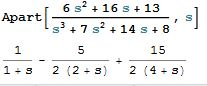
\includegraphics{Image1}}
\end{center}
We have the final transfer function as:\\
\begin{align}
G(s)=1+\bigg[\frac{-1}{s+1}+\frac{5/2}{s+2}+\frac{-15/2}{s+4}\bigg]
\end{align}
\end{section}

\begin{section}*{Part 2}
Give three different state space representations
\begin{subsection}*{a.Phase Variable (Controllable Canonical)Form}
If we have a transfer function in the form
\begin{center}
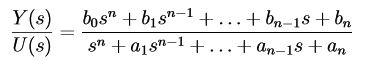
\includegraphics{Image2}
\end{center}
the state space Phase Variable form can be written as
\begin{center}
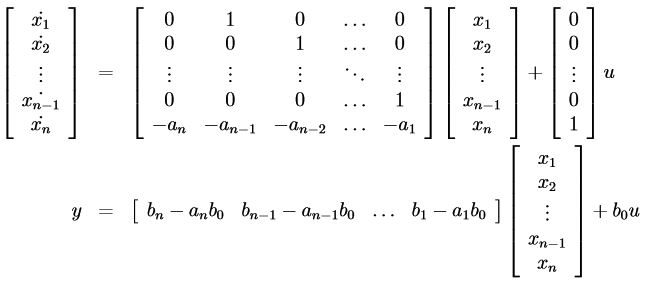
\includegraphics{Image3}
\end{center}
By inspection, the phase variable form of our specific system is

\begin{align*}
\begin{bmatrix}\dot{x_1}\\\dot{x_2}\\\dot{x_3}\end{bmatrix}=\begin{bmatrix}0 & 1 & 0\\0 & 0 & 1\\-7 & -14 & -8\end{bmatrix}\bar{x}+\begin{bmatrix}0\\0\\1\end{bmatrix}\bar{u}\\
y=\begin{bmatrix}
-13 & -16 & -6 \end{bmatrix}\bar{x} + \begin{bmatrix}1\end{bmatrix}\bar{u}
\end{align*}
\end{subsection}
\begin{subsection}*{b.Diagonal Form}
If we have a transfer function in the form
\begin{center}
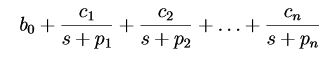
\includegraphics{Image4}
\end{center}
then the diagonal form of the state space matrices can be written as 
\begin{center}
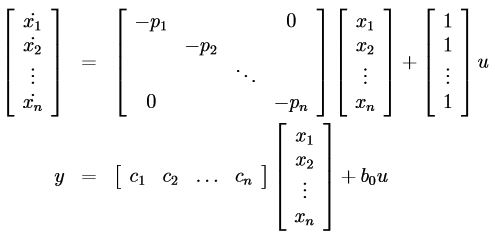
\includegraphics{Image5}
\end{center}
By inspection, the diagonal form of our state space matrix is 
\begin{align*}
\begin{bmatrix}\dot{x_1}\\\dot{x_2}\\\dot{x_3}\end{bmatrix}=\begin{bmatrix}-1 & 0 & 0\\0 & -2 & 0\\0 & 0 & -4\end{bmatrix}\bar{x}+\begin{bmatrix}1\\1\\1\end{bmatrix}\bar{u}\\
y=\begin{bmatrix}
-1 & 5/2 & -15/2 \end{bmatrix}\bar{x} + \begin{bmatrix}1\end{bmatrix}\bar{u}
\end{align*}
\end{subsection}
\begin{subsection}*{c.Any arbitrary form}
For the arbitrary form, I chose the Observable Canonical Form.  Given that the transfer function is in the form shown in Part (a) the Observable Canonical Form is expressed as
\begin{center}
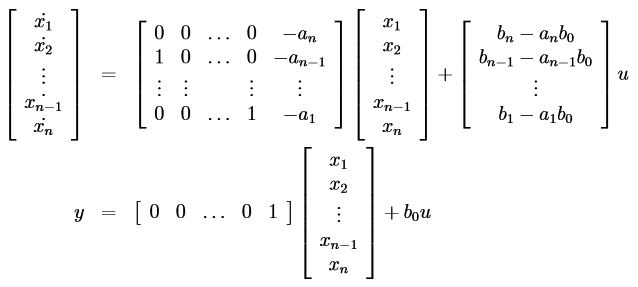
\includegraphics{Image6}
\end{center}
So by inspection, the system of interest in Observable Canonical Form is
\begin{align*}
&\begin{bmatrix}\dot{x_1}\\\dot{x_2}\\\dot{x_3}\end{bmatrix}=\begin{bmatrix}0 & 0 & -8\\1 & 0 & -14\\0 & 1 & -7\end{bmatrix}\bar{x}+\begin{bmatrix}-13\\-16\\-6\end{bmatrix}\bar{u}\\
& y=\begin{bmatrix}
0 & 0 & 1 \end{bmatrix}\bar{x} + \begin{bmatrix}1\end{bmatrix}\bar{u}
\end{align*}
The relationship between Observable and Controllable Canonical matrices are given by the properties
\begin{center}
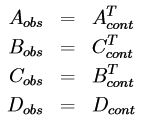
\includegraphics{Image7}
\end{center} 
\end{subsection}
\end{section}
\begin{section}*{Part 3}
Solve for y(t) when the input,u(t), is a unit step function using Laplace techniques.\\
\newline
The full Laplace transform of the differential equation is
\begin{align*}
&[s^3Y(s)-s^2y(0)-s\dot{y}(0)-\ddot{y}(0)]+7\big[s^2Y(s)-sy(0)-\dot{y}(0)]+14[sY(s)-y(0)]+8Y(s)\\=&[s^3U(s)-s^2u(0)-s\dot{u}(0)-\ddot{u}(0)]+[s^2U(s)-su(0)-\dot{u}(0)]-2[sU(s)-u(0)]-5U(s)
\end{align*}
The initial conditions are substituted into the above equation and a simplified form comes out to be
\begin{align}
Y(s)=\frac{s^3+s^2-2s-5}{s(s^3+7s^2+14s+8)}+\frac{6s+16}{s^3+7s^2+14s+8}
\end{align}
Through hand calculations, and double checking using Mathematica, a decomposed form of the out put in Laplace space is found to be
\begin{center}
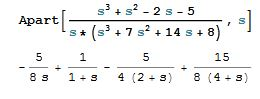
\includegraphics{Image8}\\
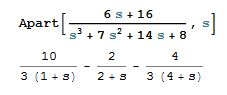
\includegraphics{Image9}\\
\end{center}
\begin{align}
Y(s)=\bigg[\frac{-5/8}{s}+\frac{1}{s+1}-\frac{5/4}{s+2}+\frac{15/8}{s+4}\bigg]+\bigg[\frac{10/3}{s+1}+\frac{-2}{s+2}+\frac{-4/3}{s+4}\bigg]
\end{align}
To get the output in the time domain, we need to take the inverse Laplace transform.
\begin{align}
y(t)=\big[-5/8+e^{-t}-5/4e^{-2t}+15/8e^{-4t}\big]+\big[10/3e^{-t}-2e^{-2t}-4/3e^{-4t}]
\end{align}
\end{section}
\begin{section}*{Part 4}
Solve for y(t) when the input,u(t),is the unit step function using state space techniques\\
We have to use the diagonal form of the state space equations from part (b), which are
\begin{align*}
\begin{bmatrix}\dot{x_1}\\\dot{x_2}\\\dot{x_3}\end{bmatrix}=\begin{bmatrix}-1 & 0 & 0\\0 & -2 & 0\\0 & 0 & -4\end{bmatrix}\bar{x}+\begin{bmatrix}1\\1\\1\end{bmatrix}\bar{u}\\
y=\begin{bmatrix}
-1 & 5/2 & -15/2 \end{bmatrix}\bar{x} + \begin{bmatrix}1\end{bmatrix}\bar{u}
\end{align*}
In order to calculate $\boldsymbol{\bar{x}(0)}$ we use the property 
\begin{align*}
\begin{bmatrix}y(0)\\\dot{y}(0)\\\ddot{y}(0)\end{bmatrix}=\begin{bmatrix}C \\ CA \\ CA^2\\\end{bmatrix}\bar{x}(0)+\begin{bmatrix}D & 0 & 0 \\CB & D & 0\\ CAB & CB & D\end{bmatrix}\begin{bmatrix}u(0)\\\dot{u}(0)\\\ddot{u}(0)\end{bmatrix}
\end{align*}
With the assistance of Mathematica, $\boldsymbol{\bar{x}(0)}$ is found to be
\begin{align}
\bar{x}(0)=\begin{bmatrix}-10/3\\-4/5\\8/45\end{bmatrix}
\end{align}
Once $\boldsymbol{\bar{x}(0)}$ has been found, the output y(t) can be found using the equation
\begin{align}
y(t)=Ce^{(At)}x(0)+C\int_{0}^{t} e^{A(t-\tau)}Bu(\tau)d\tau+Du(\tau)
\end{align}
For full calculations and intermediate steps, see attached Mathematica pages.  The end solution is found to be 
\begin{center}
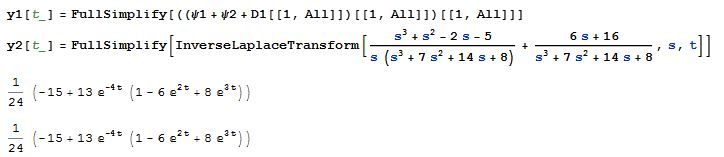
\includegraphics{Image10}
\end{center}
In order to verify similarity in solutions, the two solutions were plotted.
\begin{center}
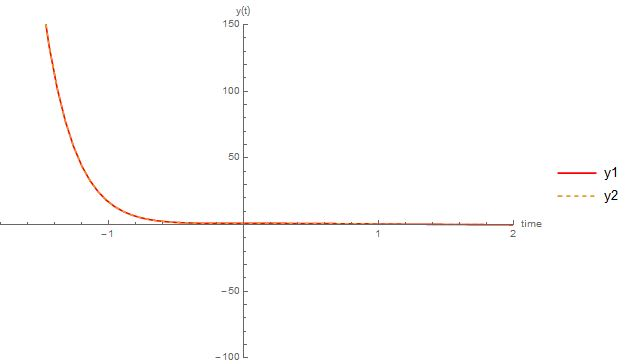
\includegraphics{Image11}
\end{center}
From the plot above, it can be seen that the solution produced by the Laplace technique is identical with the solution produced through state space methods.
\end{section}

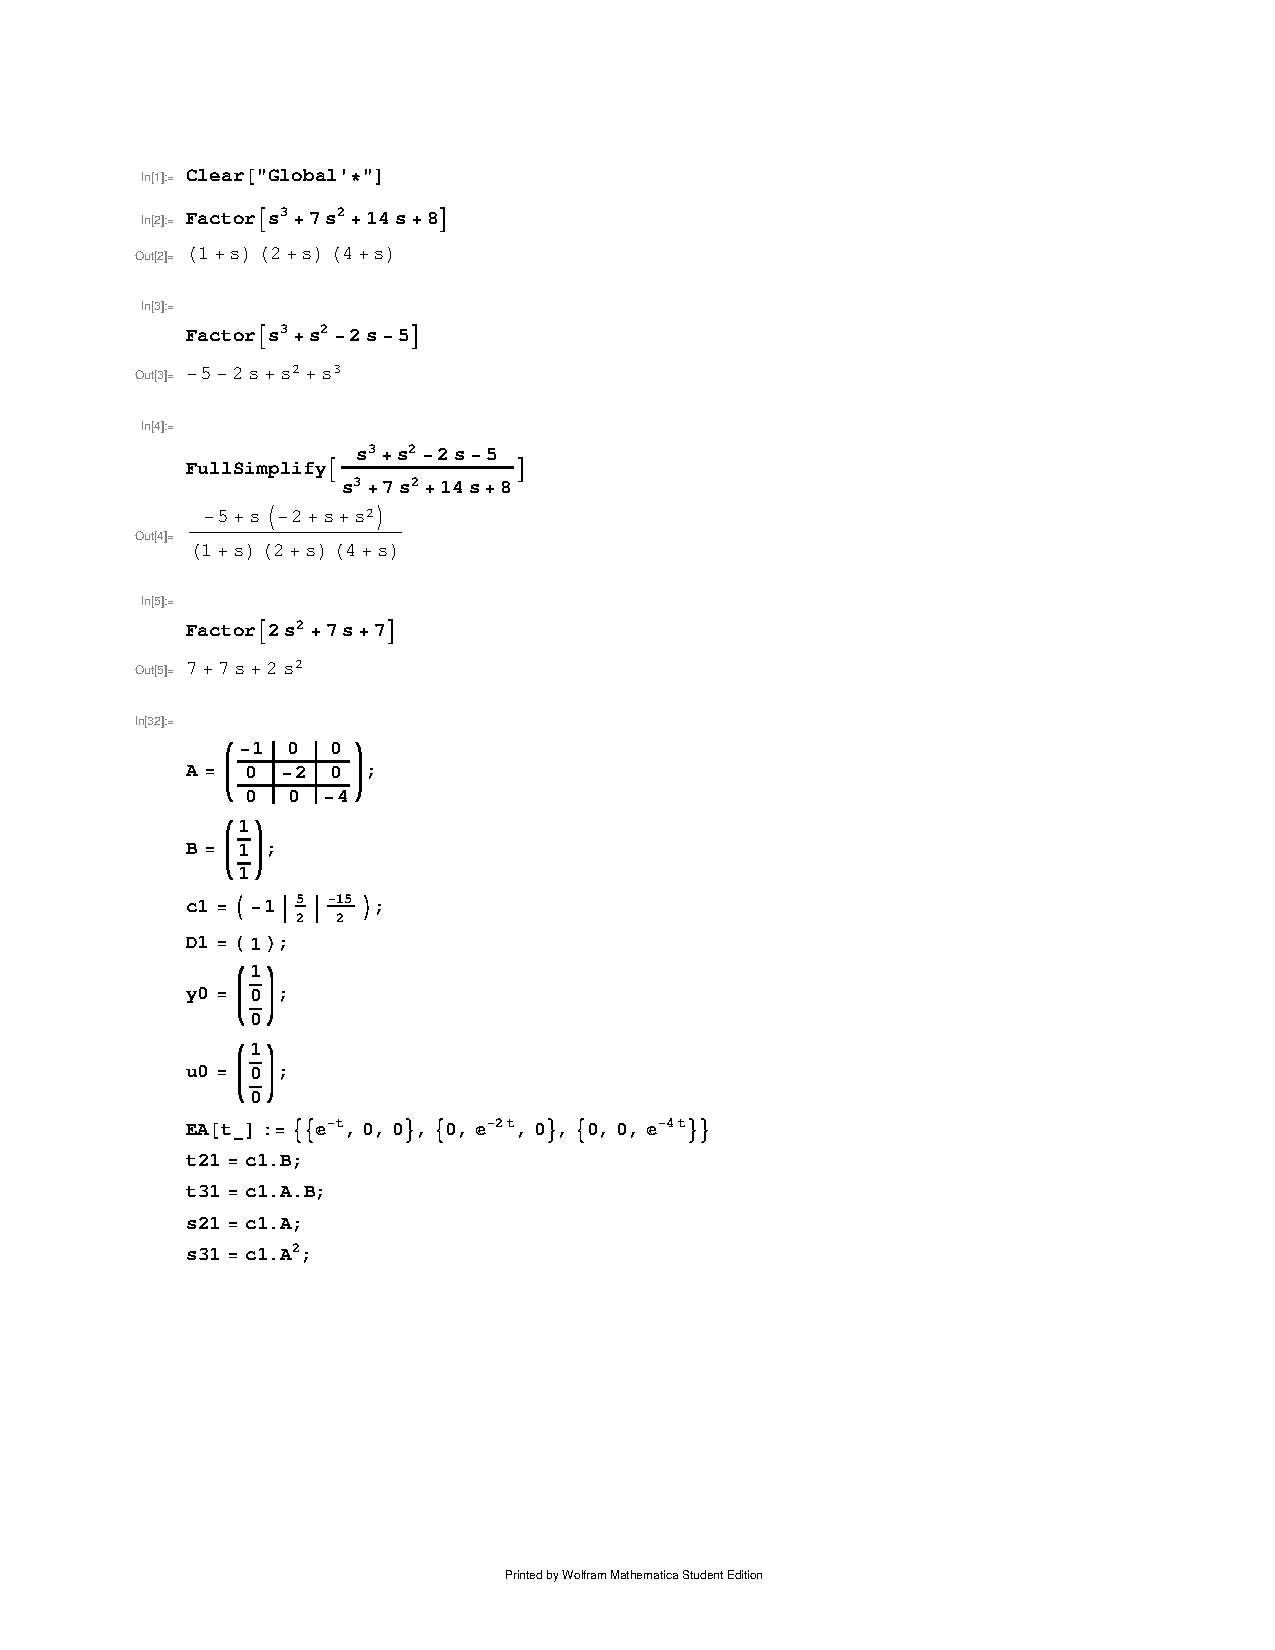
\includepdf[pages={1,2,3}]{Worksheet.pdf}


\end{document}